\section{Simulation Results}
\label{sec:simulation-results}

\subsection{Geometry and Port Configuration}

Figure~\ref{fig:cst-geometry-with-ports} shows the final vacuum region with waveguide ports on both longitudinal end faces. Figures~\ref{fig:cst-port1-setup} and \ref{fig:cst-port2-setup} document the opposite port orientations and the three-mode setting.

\begin{figure}[H]
  \centering
  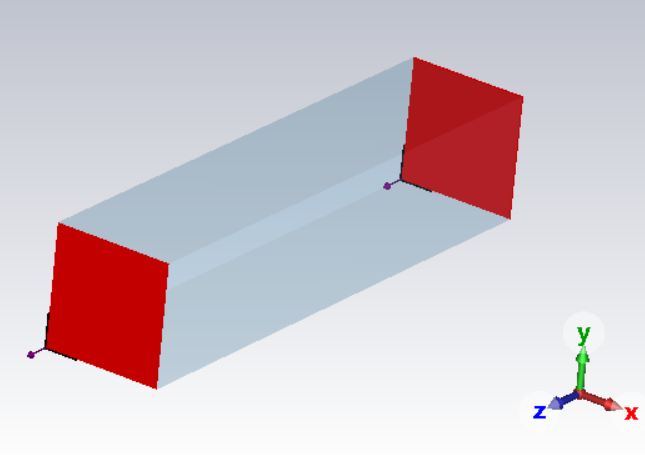
\includegraphics[width=0.65\textwidth]{figures/waveguide/fig_01_cst_geometry_with_ports.png}
  \caption{CST geometry of the \(20~\mathrm{mm}\times20~\mathrm{mm}\times90~\mathrm{mm}\) hollow guide with waveguide ports at both ends.}
  \label{fig:cst-geometry-with-ports}
\end{figure}

\begin{figure}[H]
  \centering
  \begin{subfigure}[t]{0.48\textwidth}
    \centering
    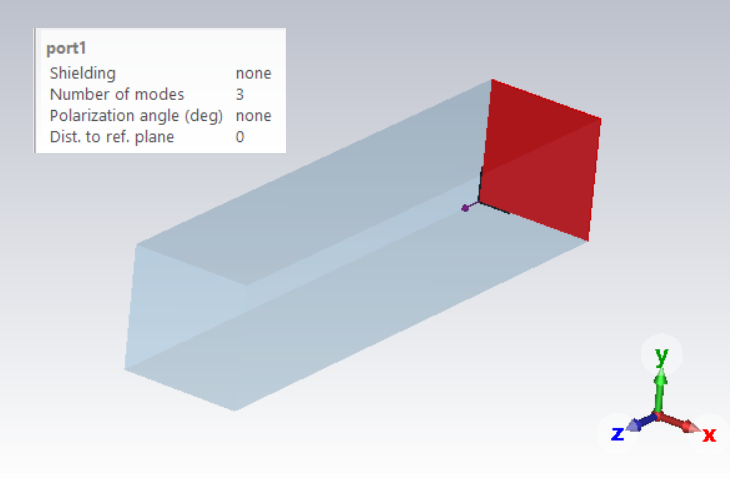
\includegraphics[width=\textwidth]{figures/waveguide/fig_02_cst_port1_z0_positive_3modes.png}
    \caption{Port 1 at \(z=0\), directed into \(+z\).}
    \label{fig:cst-port1-setup}
  \end{subfigure}
  \hfill
  \begin{subfigure}[t]{0.48\textwidth}
    \centering
    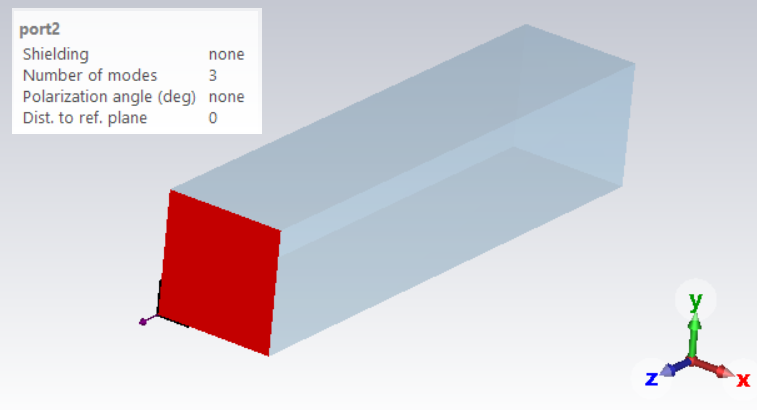
\includegraphics[width=\textwidth]{figures/waveguide/fig_03_cst_port2_z90_negative_3modes.png}
    \caption{Port 2 at \(z=90~\mathrm{mm}\), directed into \(-z\).}
    \label{fig:cst-port2-setup}
  \end{subfigure}
  \caption{Waveguide-port definitions with three solved modes per port.}
\end{figure}

\subsection{Port-Eigenmode Cutoff Frequencies}

CST reports the following cutoff frequencies:

\[
\begin{aligned}
\text{Port 1:}\quad
&7.490707,\;7.491242,\;10.5935~\mathrm{GHz},\\
\text{Port 2:}\quad
&7.49031,\;7.49064,\;10.5931~\mathrm{GHz}.
\end{aligned}
\]

Figures~\ref{fig:cst-port1-cutoff} and \ref{fig:cst-port2-cutoff} show the marked CST values.

\begin{figure}[H]
  \centering
  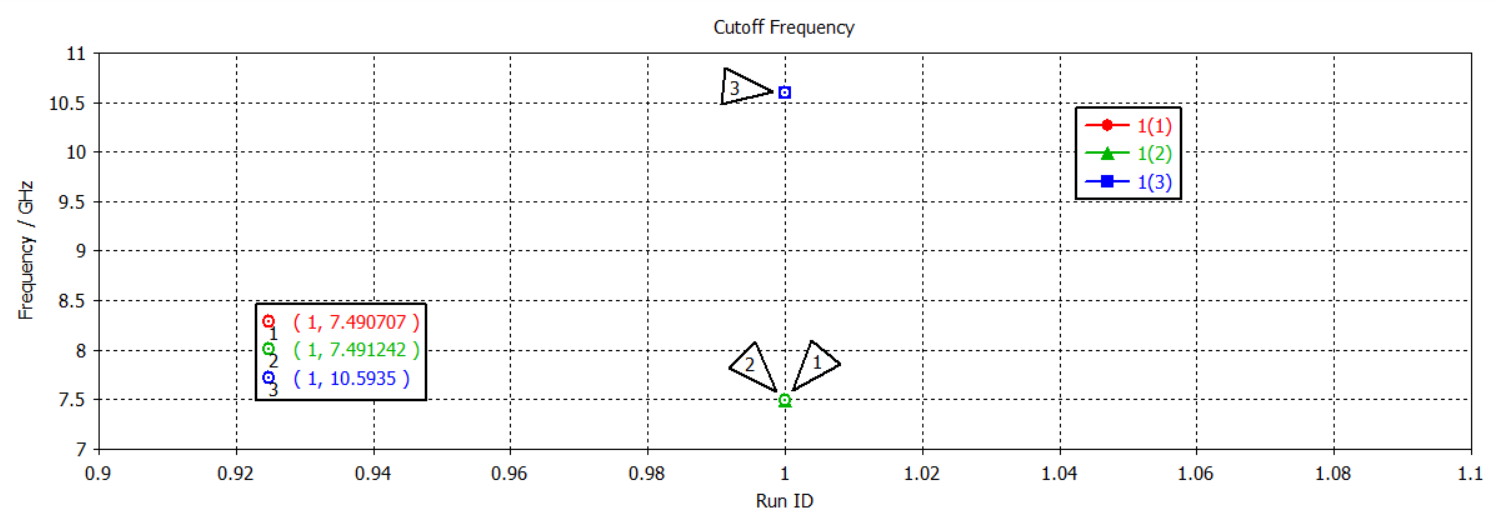
\includegraphics[width=0.92\textwidth]{figures/waveguide/fig_18_cst_port1_cutoff_frequency_first_three_modes.png}
  \caption{CST cutoff-frequency markers for the first three Port 1 eigenmodes.}
  \label{fig:cst-port1-cutoff}
\end{figure}

\begin{figure}[H]
  \centering
  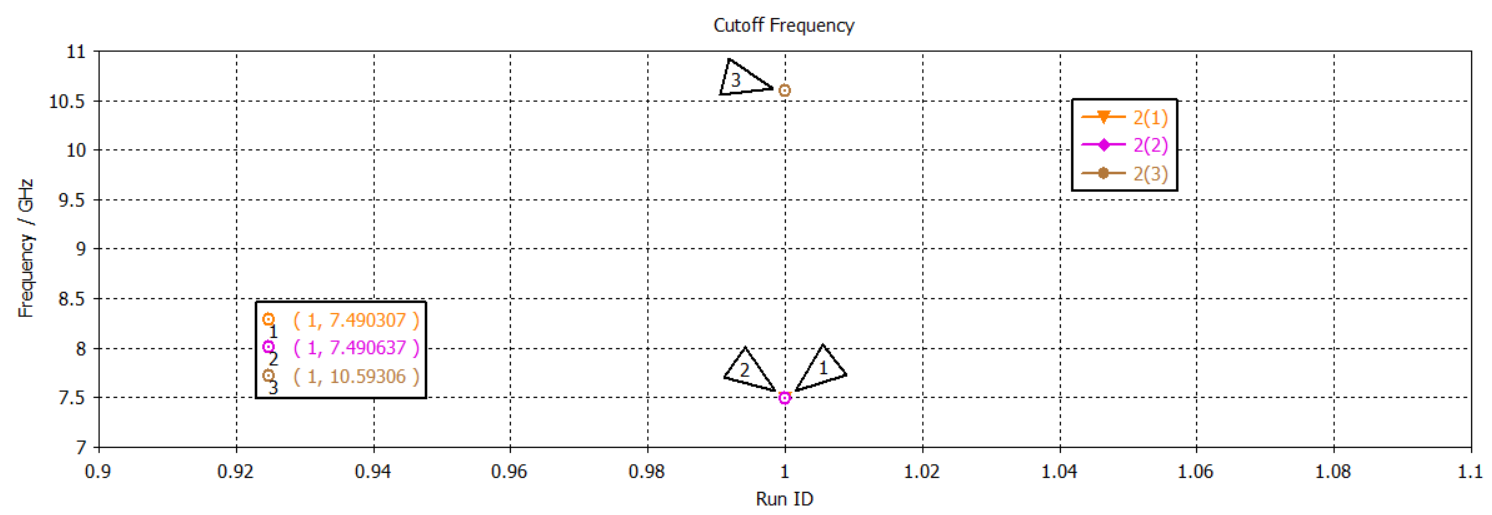
\includegraphics[width=0.92\textwidth]{figures/waveguide/fig_18d_cst_port2_cutoff_frequency_first_three_modes.png}
  \caption{CST cutoff-frequency markers for the first three Port 2 eigenmodes.}
  \label{fig:cst-port2-cutoff}
\end{figure}

\begin{table}[H]
\centering
\caption{Analytical and CST cutoff-frequency comparison.}
\label{tab:cutoff-comparison}
\resizebox{\textwidth}{!}{%
\begin{tabular}{@{}llllll@{}}
\toprule
\textbf{Solved mode} & \textbf{Theory} & \textbf{Port 1} & \textbf{Port 1 error} & \textbf{Port 2} & \textbf{Port 2 error} \\
\midrule
Mode 1 & \(7.494811~\mathrm{GHz}\) & \(7.490707~\mathrm{GHz}\) & \(-0.0548\%\) & \(7.490310~\mathrm{GHz}\) & \(-0.0601\%\) \\
Mode 2 & \(7.494811~\mathrm{GHz}\) & \(7.491242~\mathrm{GHz}\) & \(-0.0476\%\) & \(7.490640~\mathrm{GHz}\) & \(-0.0557\%\) \\
Mode 3 & \(10.599264~\mathrm{GHz}\) & \(10.593500~\mathrm{GHz}\) & \(-0.0544\%\) & \(10.593100~\mathrm{GHz}\) & \(-0.0582\%\) \\
\bottomrule
\end{tabular}%
}
\end{table}

All six differences remain below \(0.061\%\). The agreement supports the geometry definition and port-eigenmode solution.

\subsection{Modal Wave Impedance}

Figures~\ref{fig:cst-port1-impedance} and \ref{fig:cst-port2-impedance} show the frequency-dependent modal wave impedances. The first two traces are expected to overlap closely because they belong to the degenerate lowest-order TE pair.

\begin{figure}[H]
  \centering
  \begin{subfigure}[t]{0.48\textwidth}
    \centering
    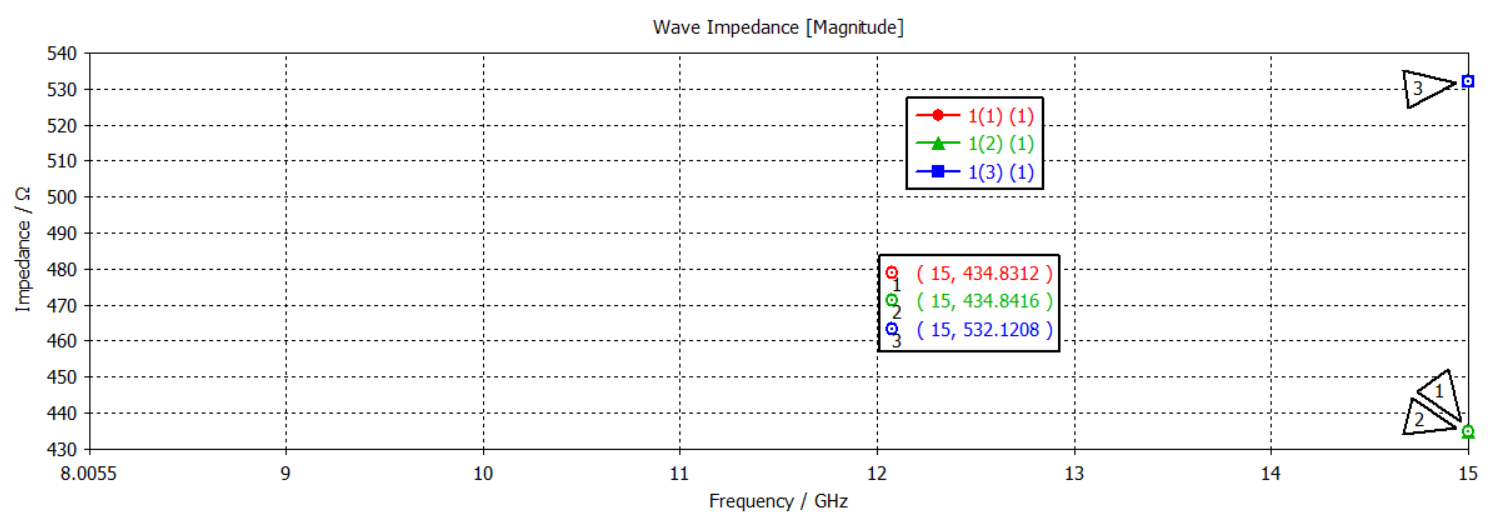
\includegraphics[width=\textwidth]{figures/waveguide/fig_19_cst_port1_wave_impedance_first_three_modes.png}
    \caption{Port 1 modal wave impedance.}
    \label{fig:cst-port1-impedance}
  \end{subfigure}
  \hfill
  \begin{subfigure}[t]{0.48\textwidth}
    \centering
    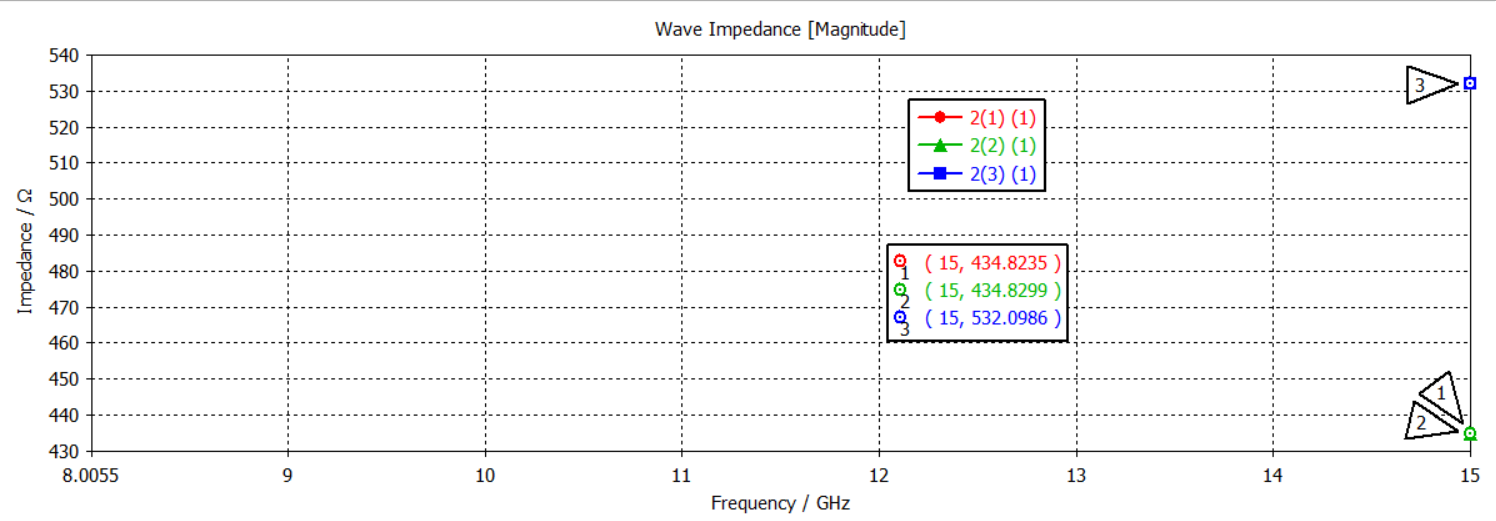
\includegraphics[width=\textwidth]{figures/waveguide/fig_20_cst_port2_wave_impedance_first_three_modes.png}
    \caption{Port 2 modal wave impedance.}
    \label{fig:cst-port2-impedance}
  \end{subfigure}
  \caption{CST wave-impedance results for the first three port eigenmodes.}
\end{figure}

The dominant analytical value at \(10~\mathrm{GHz}\) is \(569.06~\Omega\). The plots are consistent with a high TE impedance near cutoff and confirm that the ports are normalized to modal wave impedance rather than a fixed coaxial value.

\subsection{Multimode S-Parameters}

Figure~\ref{fig:cst-sparameters-all} shows the complete two-port, three-mode scattering response.

\begin{figure}[H]
  \centering
  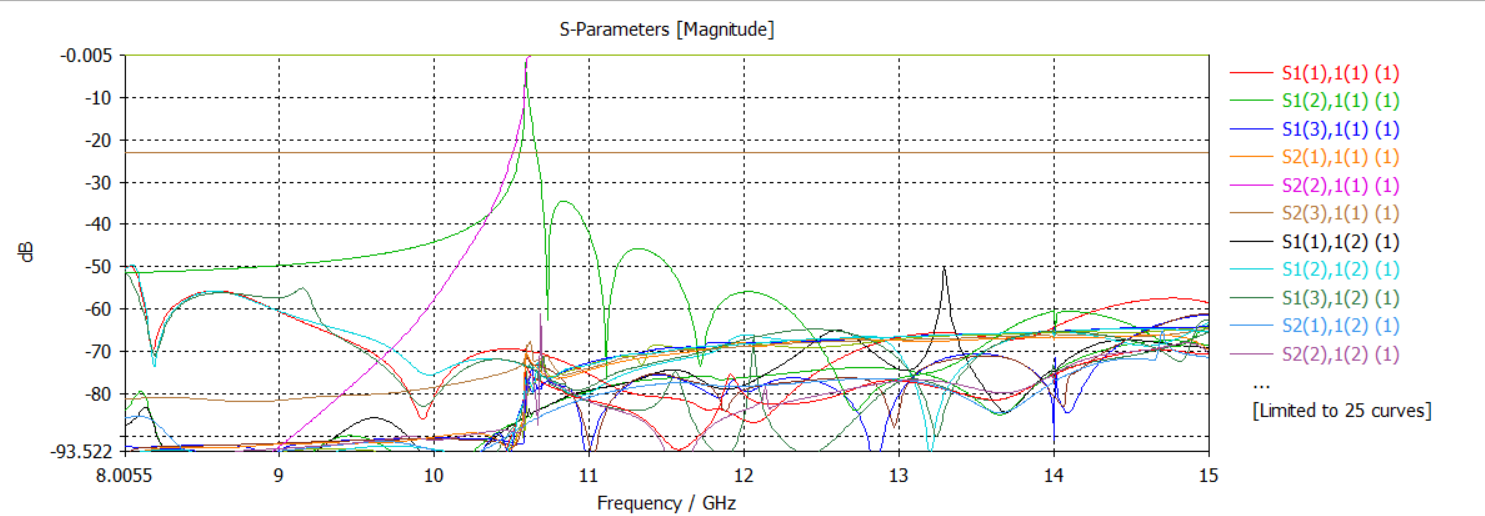
\includegraphics[width=0.92\textwidth]{figures/waveguide/fig_04_cst_sparameters_all_modal_terms.png}
  \caption{Full multimode CST S-parameter response.}
  \label{fig:cst-sparameters-all}
\end{figure}

The same-mode reflection coefficient \(S_{1(1),1(1)}\) remains below approximately \(-50~\mathrm{dB}\) across the plotted \(8\)--\(15~\mathrm{GHz}\) band and is near \(-85~\mathrm{dB}\) around \(10~\mathrm{GHz}\) by visual reading of the trace. These values are plot-derived estimates because the public package does not contain exported numerical S-parameter data.

\begin{figure}[H]
  \centering
  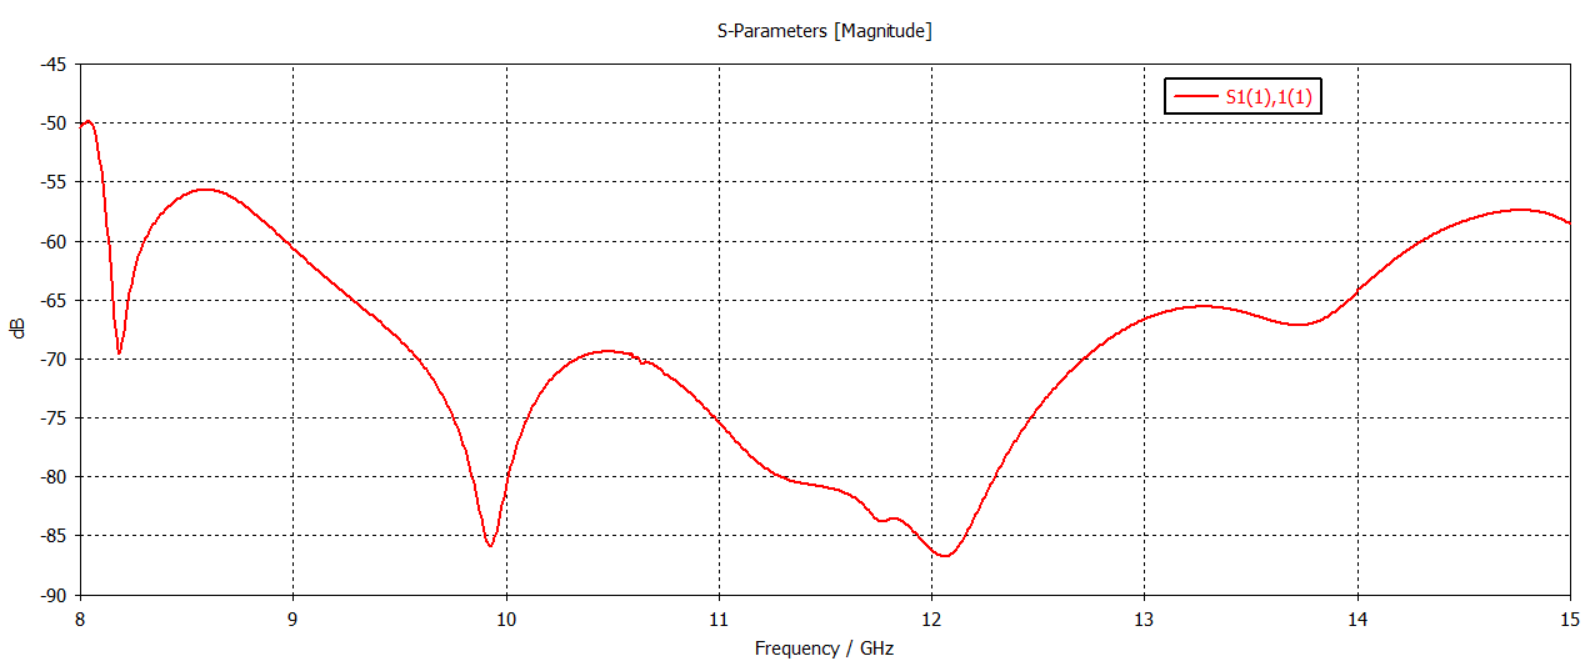
\includegraphics[width=0.90\textwidth]{figures/waveguide/fig_05_cst_s1_1_to_1_1_input_reflection.png}
  \caption{Same-mode input reflection \(S_{1(1),1(1)}\).}
  \label{fig:cst-s11-mode1}
\end{figure}

The same-index transmission term \(S_{2(1),1(1)}\) does not capture the total transmitted field because the first two modes are degenerate.

\begin{figure}[H]
  \centering
  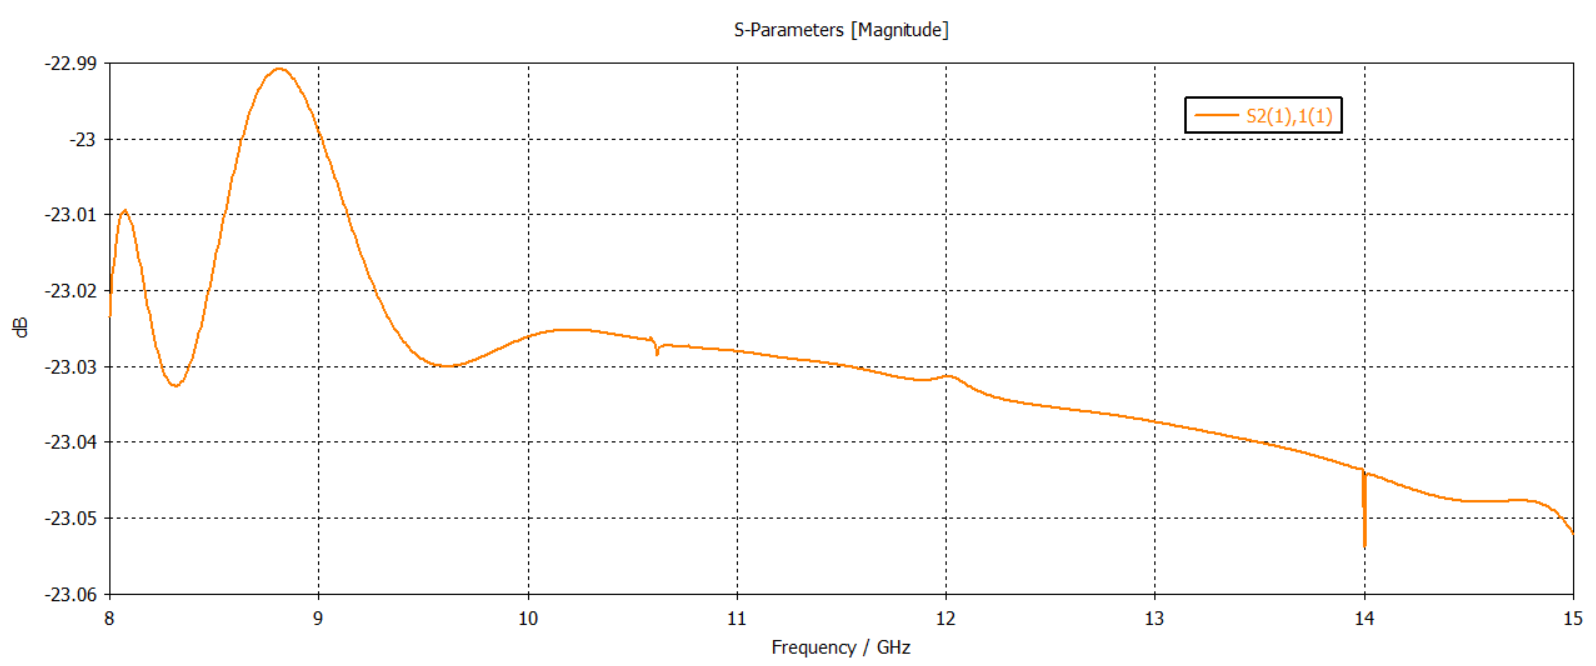
\includegraphics[width=0.90\textwidth]{figures/waveguide/fig_06_cst_s1_1_to_2_1_transmission_projection.png}
  \caption{Same-index transmission projection \(S_{2(1),1(1)}\).}
  \label{fig:cst-s21-mode1-projection}
\end{figure}

The alternate-basis coefficient \(S_{2(2),1(1)}\) stays close to \(0~\mathrm{dB}\), approximately \(-0.02~\mathrm{dB}\) near \(10~\mathrm{GHz}\) by visual reading. This is the dominant output projection.

\begin{figure}[H]
  \centering
  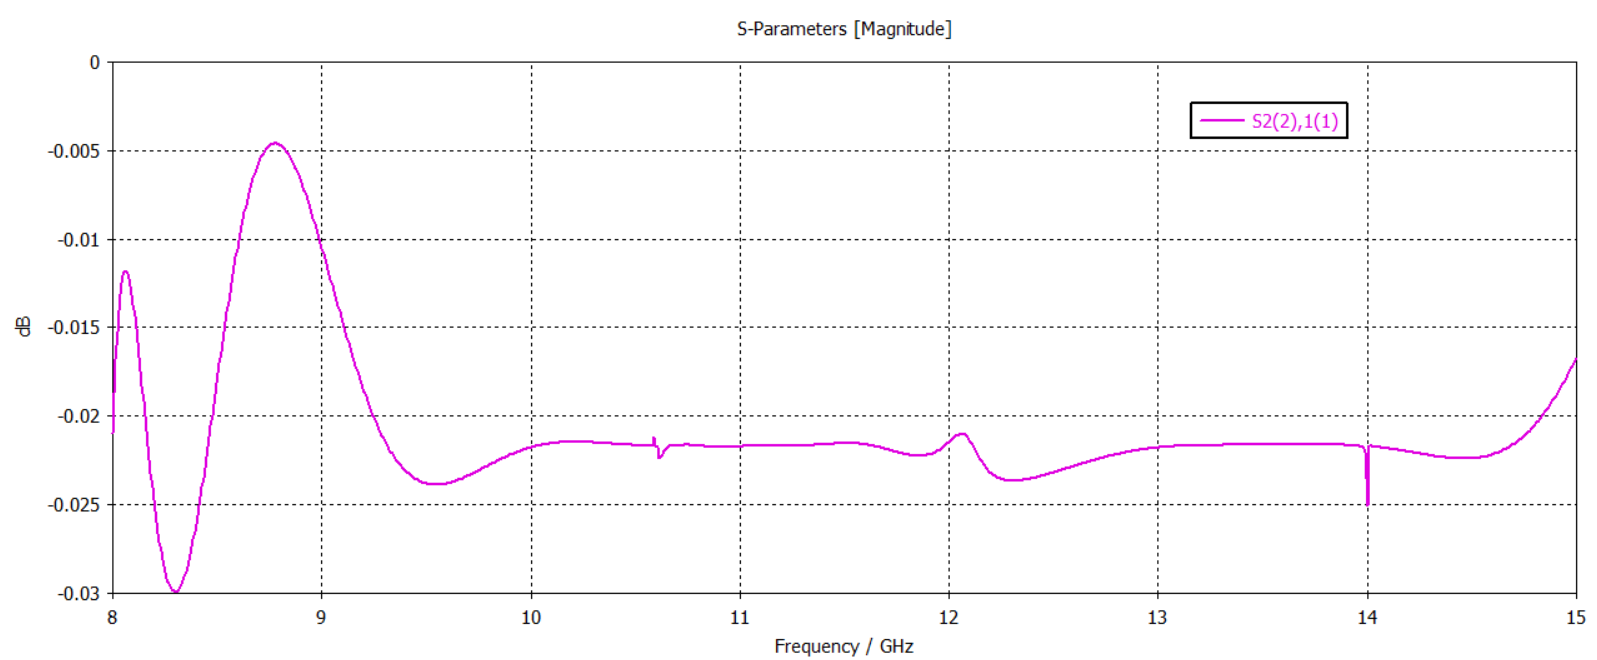
\includegraphics[width=0.90\textwidth]{figures/waveguide/fig_07_cst_s1_1_to_2_2_degenerate_transmission.png}
  \caption{Dominant transmission into the alternate member of the degenerate output basis, \(S_{2(2),1(1)}\).}
  \label{fig:cst-s21-degenerate-transmission}
\end{figure}

Coupling to the third solved output mode is much smaller.

\begin{figure}[H]
  \centering
  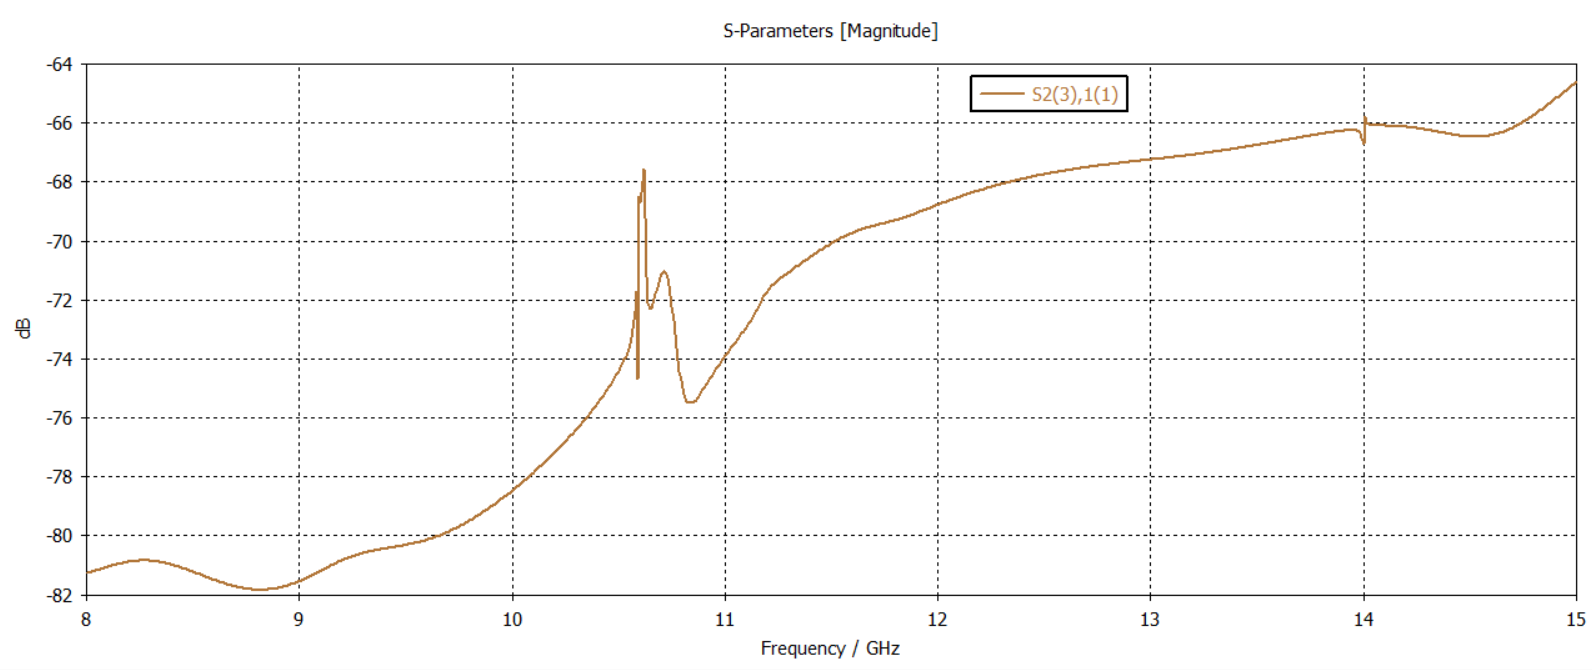
\includegraphics[width=0.90\textwidth]{figures/waveguide/fig_08_cst_s1_1_to_2_3_higher_mode_coupling.png}
  \caption{Coupling from Port 1 Mode 1 into Port 2 Mode 3, \(S_{2(3),1(1)}\).}
  \label{fig:cst-s21-higher-mode-coupling}
\end{figure}

\begin{table}[H]
\centering
\caption{Interpretation of selected multimode terms.}
\label{tab:modal-sparameter-interpretation}
\begin{tabularx}{\textwidth}{@{}lXX@{}}
\toprule
\textbf{CST term} & \textbf{Meaning} & \textbf{Interpretation} \\
\midrule
\(S_{1(1),1(1)}\) & Mode-1 input reflection & Very small in the ideal uniform guide \\
\(S_{2(1),1(1)}\) & Output Mode-1 projection & Not total transmission in a degenerate subspace \\
\(S_{2(2),1(1)}\) & Output Mode-2 projection & Dominant near-unity transmitted coefficient \\
\(S_{2(3),1(1)}\) & Third-mode projection & Weak higher-order coupling \\
\bottomrule
\end{tabularx}
\end{table}

\subsection{Electric-Field Distributions at 10 GHz}

Figures~\ref{fig:cst-efield-mode1}--\ref{fig:cst-efield-mode3} show the electric-field magnitude for excitation from the first three Port 1 modes.

\begin{figure}[H]
  \centering
  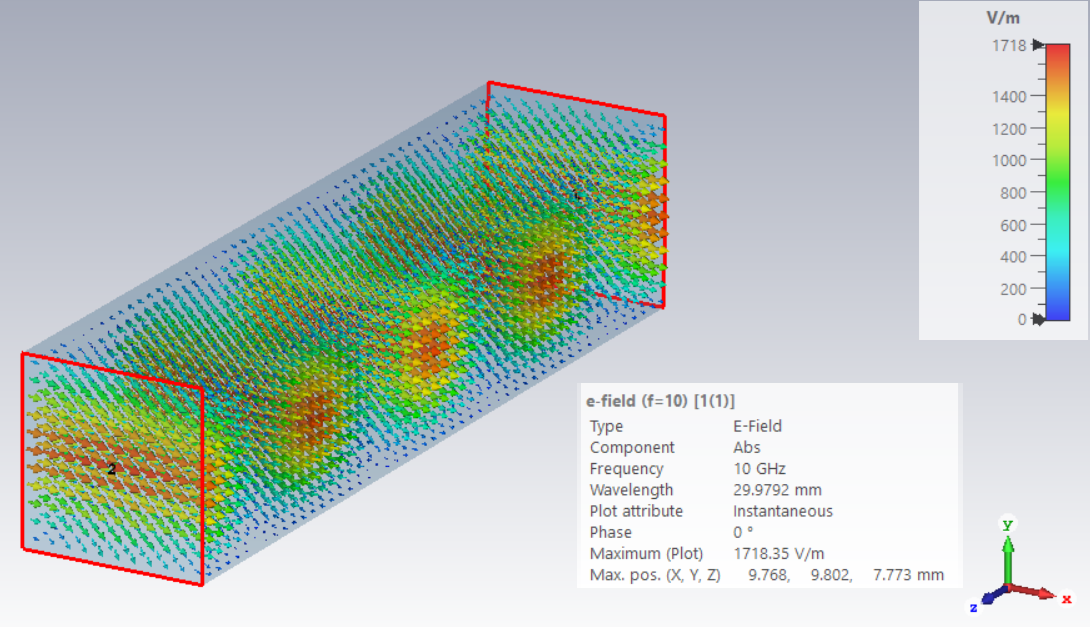
\includegraphics[width=0.88\textwidth]{figures/waveguide/fig_09_cst_efield_abs_10ghz_port1_mode1.png}
  \caption{Electric-field magnitude at \(10~\mathrm{GHz}\), Port 1 Mode 1 excitation.}
  \label{fig:cst-efield-mode1}
\end{figure}

\begin{figure}[H]
  \centering
  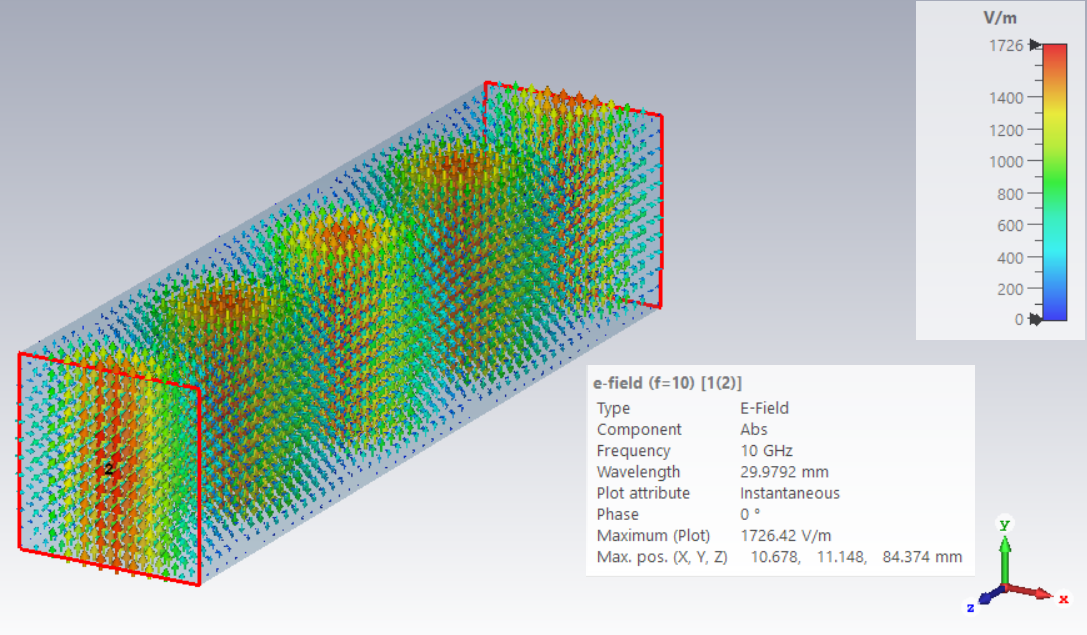
\includegraphics[width=0.88\textwidth]{figures/waveguide/fig_10_cst_efield_abs_10ghz_port1_mode2.png}
  \caption{Electric-field magnitude at \(10~\mathrm{GHz}\), Port 1 Mode 2 excitation.}
  \label{fig:cst-efield-mode2}
\end{figure}

\begin{figure}[H]
  \centering
  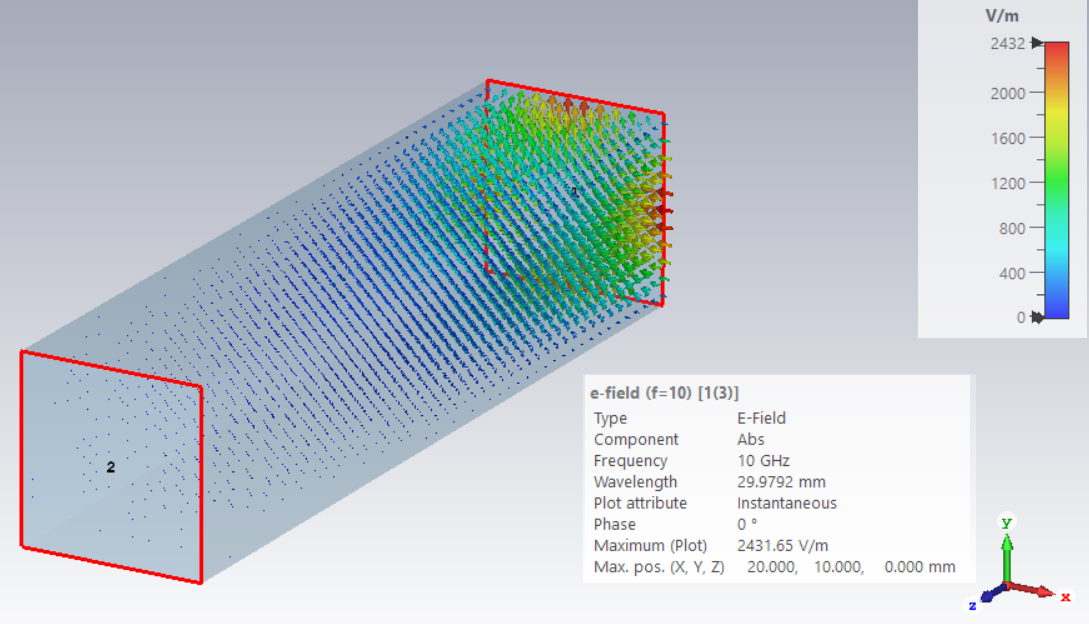
\includegraphics[width=0.88\textwidth]{figures/waveguide/fig_11_cst_efield_abs_10ghz_port1_mode3.png}
  \caption{Electric-field magnitude at \(10~\mathrm{GHz}\), Port 1 Mode 3 excitation.}
  \label{fig:cst-efield-mode3}
\end{figure}

The first two fields extend throughout the guide, consistent with propagation above cutoff. The third field is more localized because \(10~\mathrm{GHz}\) is below its \(10.5935~\mathrm{GHz}\) CST cutoff.

\subsection{Magnetic Field and Surface Current}

The magnetic-field results are shown in Figures~\ref{fig:cst-hfield-mode1}--\ref{fig:cst-hfield-mode3}. The third-mode view uses a \(270^\circ\) phase reference for visibility.

\begin{figure}[H]
  \centering
  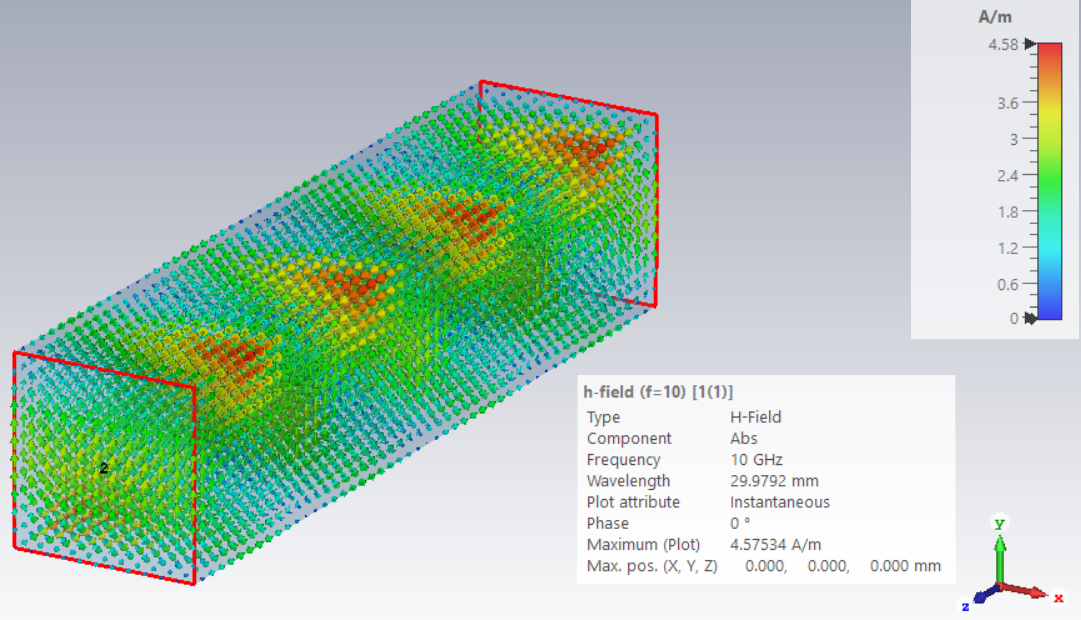
\includegraphics[width=0.88\textwidth]{figures/waveguide/fig_12_cst_hfield_abs_10ghz_port1_mode1.png}
  \caption{Magnetic-field magnitude at \(10~\mathrm{GHz}\), Port 1 Mode 1 excitation.}
  \label{fig:cst-hfield-mode1}
\end{figure}

\begin{figure}[H]
  \centering
  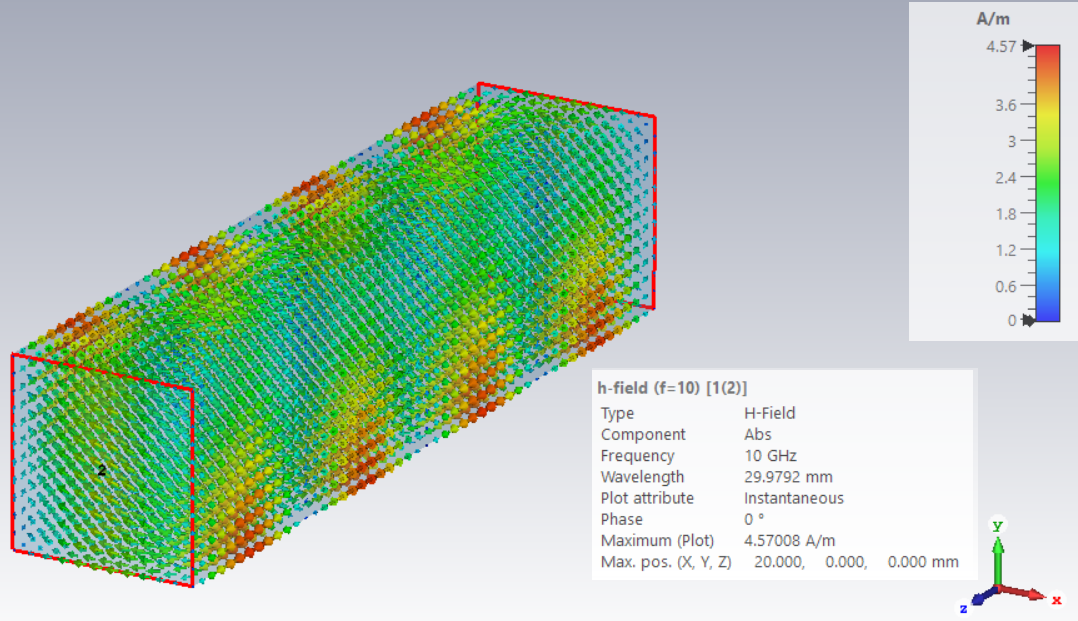
\includegraphics[width=0.88\textwidth]{figures/waveguide/fig_13_cst_hfield_abs_10ghz_port1_mode2.png}
  \caption{Magnetic-field magnitude at \(10~\mathrm{GHz}\), Port 1 Mode 2 excitation.}
  \label{fig:cst-hfield-mode2}
\end{figure}

\begin{figure}[H]
  \centering
  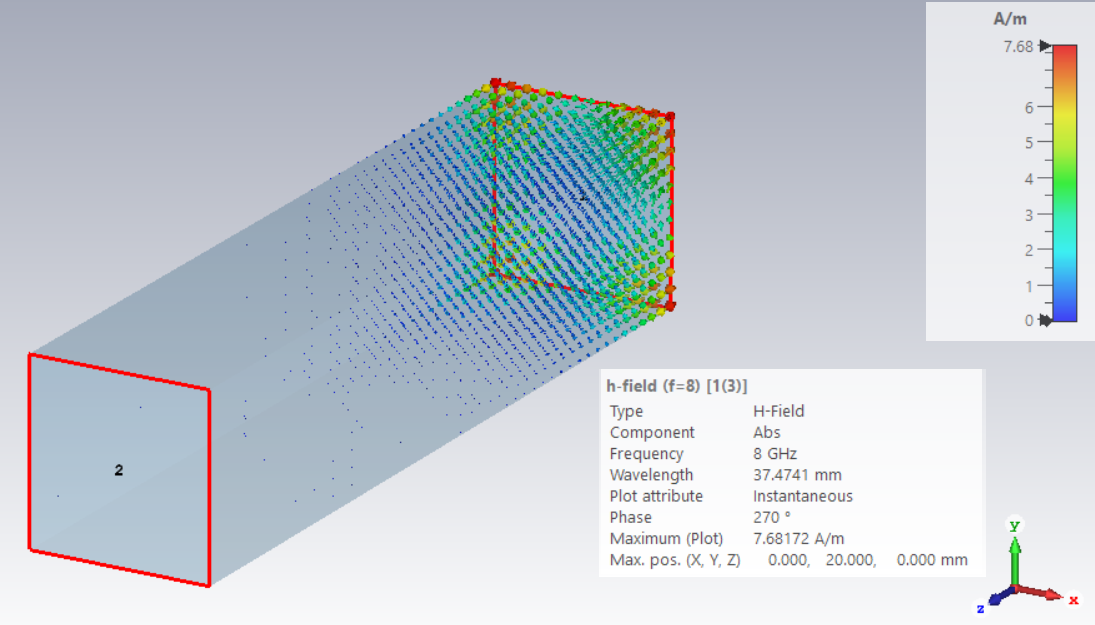
\includegraphics[width=0.88\textwidth]{figures/waveguide/fig_14_cst_hfield_abs_10ghz_port1_mode3_phase270.png}
  \caption{Magnetic-field magnitude at \(10~\mathrm{GHz}\), Port 1 Mode 3 excitation, displayed at \(270^\circ\) phase.}
  \label{fig:cst-hfield-mode3}
\end{figure}

Figures~\ref{fig:cst-current-mode1}--\ref{fig:cst-current-mode3} show the corresponding wall-current distributions induced by the modal fields.

\begin{figure}[H]
  \centering
  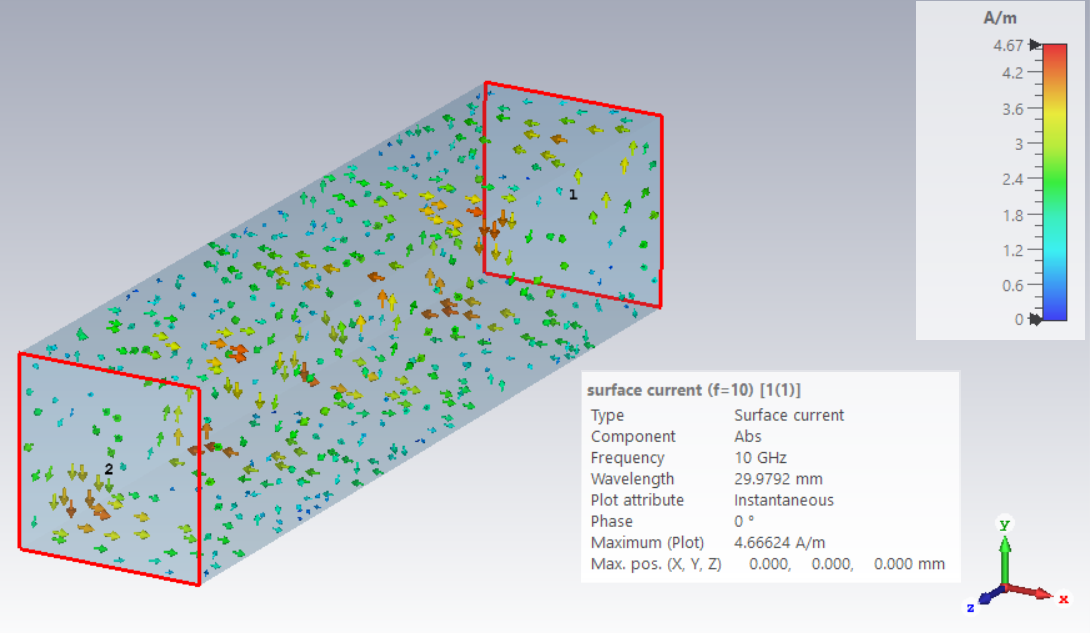
\includegraphics[width=0.88\textwidth]{figures/waveguide/fig_15_cst_surface_current_abs_10ghz_port1_mode1.png}
  \caption{PEC wall-current magnitude at \(10~\mathrm{GHz}\), Port 1 Mode 1 excitation.}
  \label{fig:cst-current-mode1}
\end{figure}

\begin{figure}[H]
  \centering
  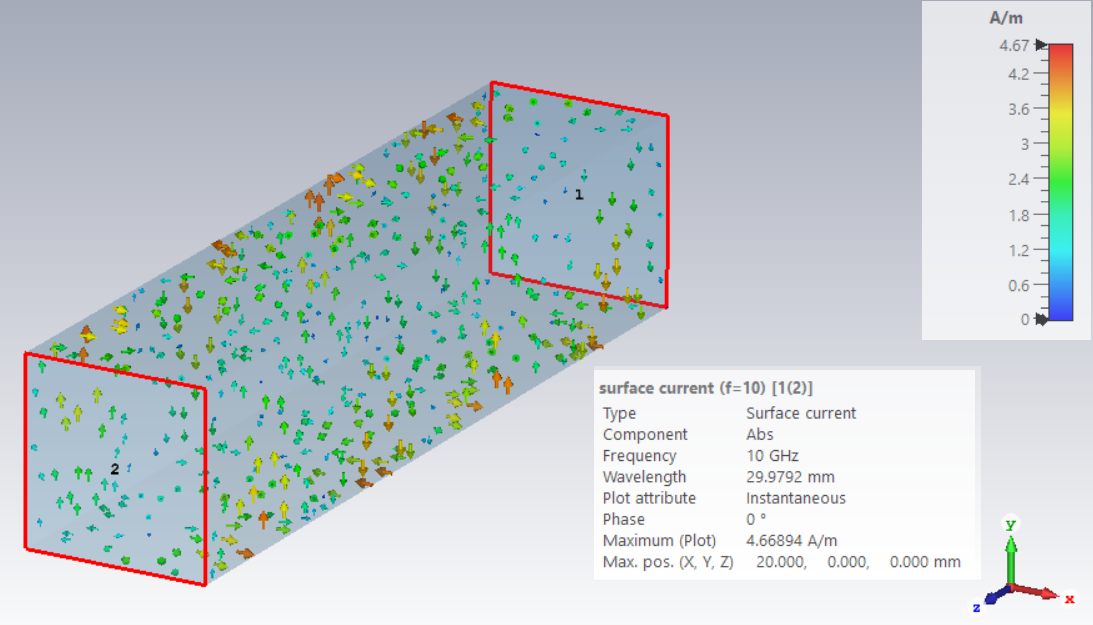
\includegraphics[width=0.88\textwidth]{figures/waveguide/fig_16_cst_surface_current_abs_10ghz_port1_mode2.png}
  \caption{PEC wall-current magnitude at \(10~\mathrm{GHz}\), Port 1 Mode 2 excitation.}
  \label{fig:cst-current-mode2}
\end{figure}

\begin{figure}[H]
  \centering
  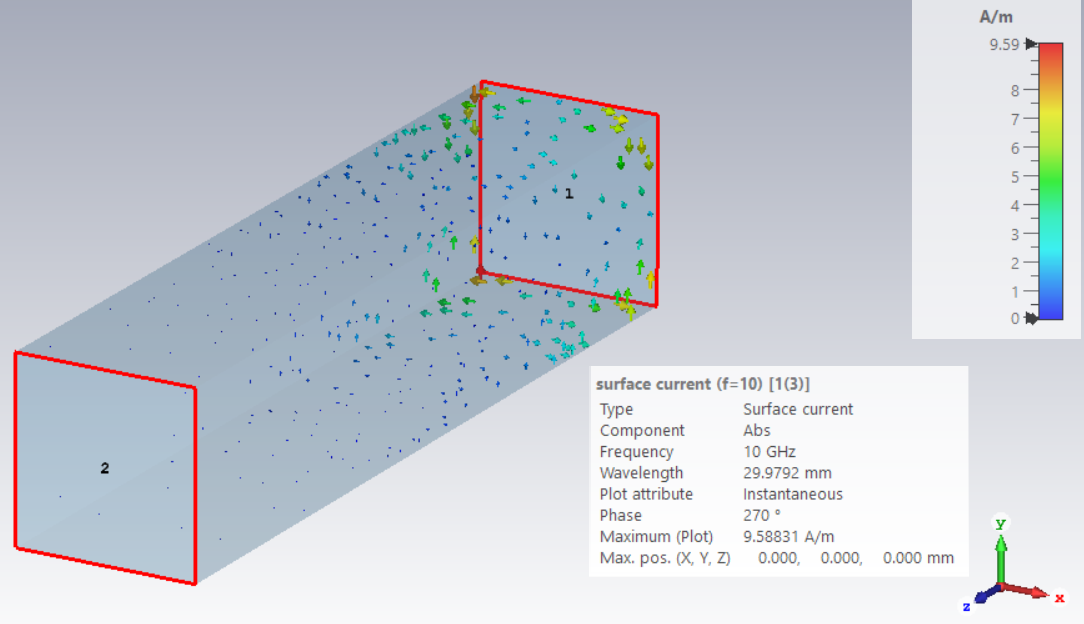
\includegraphics[width=0.88\textwidth]{figures/waveguide/fig_17_cst_surface_current_abs_10ghz_port1_mode3_phase270.png}
  \caption{PEC wall-current magnitude at \(10~\mathrm{GHz}\), Port 1 Mode 3 excitation, displayed at \(270^\circ\) phase.}
  \label{fig:cst-current-mode3}
\end{figure}
